% Fig. 3.12 -- the slice of the joint pdf has to be divided by the marginal
%   density before it is a legitimate pdf.
% Source: mathstatch3.tex lines 1349-1392 (a plain tikzpicture, not pgfplots).
%
% The manuscript draws two bell curves of one and the same shape,
%   3 e^{-(x-4)^2/3}   (peak 3, shaded underneath, labelled f_XY(x,1.5))
%   4.5 e^{-(x-4)^2/3} (peak 4.5, unshaded, labelled f_X|Y(x|1.5)),
% so the taller one is 1.5 times the shorter one; the shorter one is the raw
% slice and the taller one is that slice divided by f_Y(1.5).  Two leader
% lines carry the labels, one up-left off the taller curve and one up-right
% off the shorter one.
%
% Per CH2_FIGURE_SPECS.md 1.6 the web version replaces the manuscript's
% schematic curves by a genuine density, so that the upper curve really does
% enclose area 1 and the lower one really is the smaller multiple of it:
%   f_X|Y(x|1.5) = 0.3989423 e^{-(x-2.8)^2/2}            (area 1)
%   f_XY(x,1.5)  = (2/3) f_X|Y(x|1.5)                    (area 2/3)
% The factor 2/3 is the manuscript's own 3 : 4.5 ratio read the other way
% round, i.e. the picture is drawn for f_Y(1.5) = 2/3.  Over the plotted
% range 0 <= x <= 6.4 the upper curve encloses 0.99521 rather than 1, the
% remainder being the two tails outside the range; the ratio of the two
% curves is exact everywhere.
%
% Drawing scale x = 0.95cm, y = 7.6cm.  Peaks: upper 3.03196cm, lower
% 2.02131cm.  Leader feet: upper curve at x = 2.05 (height 2.28864cm),
% lower curve at x = 4.43 (height 0.53542cm).
%
% Deviations from the manuscript picture:
%
% 1. The leader lines are shortened from the manuscript's 1 unit right and
%    1 unit up (about 1.41cm on the diagonal) to 0.55cm and 0.52cm, and the
%    left-hand label is hung on the leader's own end rather than a further
%    node width to its left.  At the manuscript's length the left label
%    would stand 1.4cm clear of the drawing and the bounding box would grow
%    to about 8.6cm wide, at which width the scriptscript subscripts fall to
%    11.3px at the 350px phone width, against the 11px floor of
%    CH3_FIGURE_SPECS.md section 1.
%
% 2. \DeclareMathSizes{10}{10}{9}{8} raises the math script sizes from the
%    default 7pt/5pt, as CH2_FIGURE_SPECS.md 1.3 requires wherever \sssig
%    appears.  Native size 213.56 x 95.265 pt (drawing 7.37cm wide).  A mark
%    of S pt shows at S x 0.99626 x <display width> / 213.56 px, so at the
%    350px phone width of a topic-figure--wide in body text
%        10pt text 16.33px, 9pt scripts 14.69px, 8pt scriptscripts 13.06px
%    and at the 620px desktop width 28.92 / 26.03 / 23.14px.
%
% 3. The leader off the shorter curve crosses the taller curve at about
%    x = 4.6, where the taller curve stands at 0.60cm, i.e. one fifth of its
%    own peak.  The manuscript's leader crosses at the same relative height;
%    any leader off the lower of two nested curves has to cross the upper
%    one, since the lower curve lies under it everywhere.
\documentclass[tikz,border=2pt]{standalone}
\usepackage{amsmath}
\usepackage{amssymb}
\usepackage{xcolor}
\usetikzlibrary{arrows.meta}
\newcommand{\sssig}{\scriptscriptstyle}
\DeclareMathSizes{10}{10}{9}{8}

\definecolor{journalink}{HTML}{1F1C18}
\definecolor{journalmuted}{HTML}{8A7F72}
\definecolor{journalaccent}{HTML}{9C2D2D}

\begin{document}
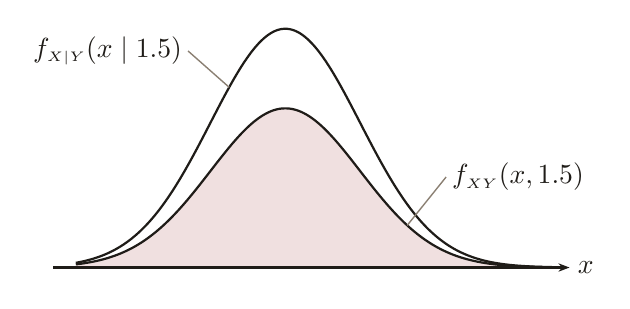
\begin{tikzpicture}[
  x=0.95cm,
  y=7.6cm,
  every node/.style={font=\normalsize, journalink},
  axis/.style={journalink, line width=0.8pt, -{Stealth[length=4pt]}},
  curve/.style={journalink, line width=0.8pt},
  leader/.style={journalmuted, line width=0.5pt},
  region/.style={journalaccent, fill opacity=0.15}
]
  % ---- the raw slice, shaded underneath -------------------------------
  \fill[region]
    (0,0) -- (6.4,0) -- (6.4,0.0004079)
    -- plot[domain=6.4:0, samples=200, smooth]
       (\x,{0.2659615*exp(-(\x-2.8)*(\x-2.8)/2)})
    -- cycle;

  % ---- the two curves --------------------------------------------------
  % lower: the slice f_XY(x, 1.5), area 2/3
  \draw[curve] plot[domain=0:6.4, samples=200, smooth]
    (\x,{0.2659615*exp(-(\x-2.8)*(\x-2.8)/2)});
  % upper: the conditional pdf f_X|Y(x|1.5), area 1
  \draw[curve] plot[domain=0:6.4, samples=200, smooth]
    (\x,{0.3989423*exp(-(\x-2.8)*(\x-2.8)/2)});

  % ---- x axis ----------------------------------------------------------
  \draw[axis] (-0.3,0) -- (6.6,0);
  \node[anchor=west, inner sep=2.8pt] at (6.6,0) {$x$};

  % ---- label on the conditional pdf, leader up-left --------------------
  \draw[leader] ([yshift=2.28864cm]2.05,0) -- ([yshift=2.75cm]1.50,0);
  \node[anchor=east, inner sep=2pt] at ([yshift=2.75cm]1.50,0)
    {$f_{\sssig X\mid Y}(x\mid 1.5)$};

  % ---- label on the raw slice, leader up-right -------------------------
  \draw[leader] ([yshift=0.53542cm]4.43,0) -- ([yshift=1.15cm]4.95,0);
  \node[anchor=west, inner sep=2pt] at ([yshift=1.15cm]4.95,0)
    {$f_{\sssig XY}(x,1.5)$};
\end{tikzpicture}
\end{document}
